\section{Measurements and Tests}
% Laser: KY 008
% Photo Resistor: KY
This chapter covers the power drain from the sensor, laser and the esp32, inlcuding deepsleep and bluetooth, to determine the optimal setup. The measurement or test setup is explained in each respective section. The tests are guiding points and are not intended for scientific or statisitcal significance. Their goal is to provide an order of magnitude of the power consumption of the individual components to guide future architectural decisions. This chapter will first look at the laser and sensor measurments and afterwards at the power consumption of normal/idle and deepsleep and then how much a wake up from deepsleep costs and transmitting data.


\subsection{Laser}
We measured the laser on a power source directly connected to the esp32 which has an output rating of $4.695V$ with a max current of $80mA$. The laser consumed on average $25mA$ and thus the power consumption is
\begin{equation*}
    4.695V * 25mA = 0.117W
\end{equation*}
which is, as expected, fairly high. In a setup with to lasers per goal, this could be a realy problem


\subsection{Sensor}
Next, we measured the power consumption of the sensor, again powered by the esp32, so $4.695V$ with a max current of $80mA$. It consumed on average $3.5mA$ when the laser was hitting the sensor and $3.8mA$ when it was not. As the default state is hitting and only goals, so very short periods, are not hitting, the power consumption is
  \begin{equation*}
      4.695V * 3.5mA = 0.016W.
    \end{equation*}
This is inline with the expectations, as the resistance drops when the laser hits the sensor. 
To summarize, together the sensor and laser consume around  
\begin{equation*}
    0.016W + 0.117W = 0.133W
  \end{equation*}
in idle and a little bit more when a goal is scored. Thus the power consumption in one day is
\begin{equation*}
    0.133W * 24 = 3.19Wh
\end{equation*}
This is quite a lot especially running on a battery with only
\begin{equation*}
    0.133W * 24 = 12Wh
\end{equation*}

\subsection{ESP32 Modes and BLE}
The esp32 development board from wemos consumes around $43mA$ in idle and $0.014mA$ in deepsleep. This is much higher than esp32 wroom board which is supposed to only consume $20mA$ in idle and $0.01mA$ in deepsleep\cite{InsightI15esp32ModesWroom:online}. \Cref{fig:esp32Comp} shows both microcontrollers side by side. 

\begin{figure}[h!]
    \centering
    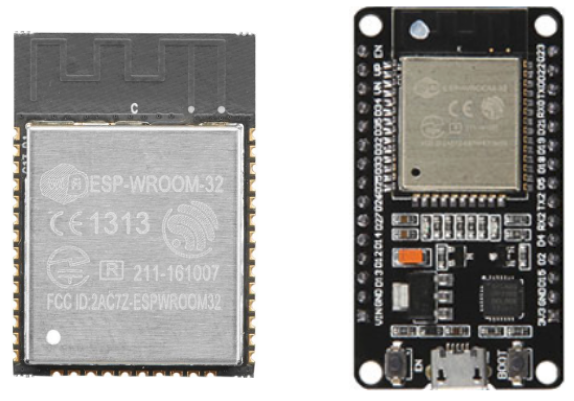
\includegraphics[scale=0.4]{figures/esp32WroomWemos.png}% picture filename
    \caption{ESP32 wroom (left) and Wemos development board (right).}\label{fig:esp32Comp}
\end{figure}



The development board has a microusb controller and additional current controls and a power LED. These extra components add up to the significant power consumption difference. For the production we thus plan on using a esp32 Wroom and soldier the connections ourselfs. Thus, instead of using our numbers we will use the numbers from the esp32 wroom controller\cite{InsightI15esp32ModesWroom:online}.\\

The power consumption also changes during boot time and during data transmission. In the former, the processor consumes a lot of power, while in the latter, the radio chip, including antenna, consumes the majority of extra power. Unfortuately, we were not able to get a esp32 wroom in time for the tests, so we have to infere values from the esp32 wemos development board. \\

In our tests, waking up from deepsleep took around $250ms$ and increased current consumption to about $80mA$\footnote{This was done via eye measurment with a lot of fluctations, so the numbers are really only approximates.}. Especially, the wake up time seems quite slow and we would like to test this further and search for wake up optimizations in further research.
During the initialization of the bluetooth radio power consumption was similar to the wake up, again showing that the processor is tasked more heavily. Sending and receiving of data, the power consumption increased to $50mA$ but for such short time periods that in our calculation we omit sending information. Unfortuately, we did not have the time to test how much power it cost to act as a slave and search for ble beacons and receive data.\\


To summarize in idle the esp32 consumes
\begin{equation*}
    0.02A * 5V *1h= 0.1Wh
\end{equation*}
while each wake up costs
\begin{equation*}
    0.08A * 5V *1h= 0.4Wh
\end{equation*}
per hour so for a startup time of $\frac{1}{3}s$  that constitutes to 
\begin{equation*}
    0.4Wh / (3600 / \frac{1}{3}) = 0.000037W = 0.037mW
\end{equation*}
Initializing the bluetooth radio is fast at around $\frac{1}{10}s$ and consumes 
\begin{gather*}
        0.08A * 5V * 1h = 0.4Wh \\
        0.4Wh / (3600 / \frac{1}{10}) = 0.000011W = 0.011mW 
\end{gather*}

\subsection{Summary}
Together the laser and sensor consume $0.133W$. The esp32 consumes $0.01mA$ in deepsleep and $20mA$ in idle. It spikes at around $80mA$ for initialization periods which total $\frac{4.3}{10}s$ and thus each start costs $0.048mW$.
